\chapter{Présentation du projet}

%Intro\footnotemark\\
%note en bas de page

\section{Sujet}
Le sujet ne peut être abordé sans un rapide point sur les différents aspects de la logique du premier ordre telle qu'elle sera utilisée dans le projet:

\subsection{Introduction à la logique du premier ordre}
Une formule de la logique des prédicats, telle qu'elle sera écrite par
les étudiants, est constituée de termes, de prédicats, de
quantificateurs et de connecteurs logiques. Prenons par exemple la
formule suivante :

\begin{center}
	$ \forall x Rose(x) \Rightarrow estRouge(x) $
\end{center}

Pour écrire une telle formule, l'étudiant utilise des termes comme
briques de base. Ces termes correspondent soit à l'ensemble $F_0=\{a,
b, ..., t\}$ des constantes, soit à l'ensemble $X=\{v, w, x, y, z\}$
des variables.  \newline Ensuite, il dispose également d'un ensemble
de prédicat $P_i$ d'arité $i$, pour $i\in \{1,2,3\}$. Chaque prédicat
de $P_1, P_2, P_3$ prend ainsi respectivement 1, 2 ou 3 termes en
argument. Dans notre exemple, $Rose(x)$ et $estRouge(x)$ sont deux
prédicats de $P_1$ et prennent la variable $x$ en argument.  \newline
\`A partir de ces formules de base, l'ensemble des formules est défini
inductivement : si $\varphi$ est une formule alors $\lnot \varphi$ est
également une formule. De même si $\varphi_1$ et $\varphi_2$ sont des
formules alors $\varphi_1 \land \varphi_2$, $\varphi_1 \lor \varphi_2$
et $\varphi_1 \Rightarrow \varphi_2$ aussi.  Enfin, si $x \in X$ et
$\varphi$ est une formule alors $\forall x \varphi$ et $\exists x
\varphi$ aussi.  \newline Ce projet utilise un ensemble de prédicat
prédéfinis que l'on regroupera par arité :
\begin{itemize}
	\item[\textit{Unaire}] définissant l'état d'une fleur, elle peut être :
		\begin{itemize}
			\item une rose, une paquette ou une tulipe
			\item petite, moyenne ou grande
			\item rouge, rose ou blanche
			\item à l'est, à l'ouest, au sud ou au nord
		\end{itemize}
              \item[\textit{Binaire}] définissant une relation entre 2
                fleurs, la fleur $a$ peut être :
		\begin{itemize}
                \item à l'est, à l'ouest, au sud ou au nord de la
                  fleur $b$
			\item à la même latitude ou longitude que la fleur $b$
			\item plus grande, plus petite ou de même
                          taille que la fleur $b$
			\item de la même couleur que la fleur $b$
		\end{itemize}
              \item[\textit{Ternaire}] définissant une relation entre
                3 fleurs, la fleur $c$ peut être :
		\begin{itemize}
                \item entre la fleur $a$ et la fleur $b$
		\end{itemize}
\end{itemize}

La section suivante présente quelques exemples de formules utilisant
différents prédicats.

\subsection{Exemple}

On peut par exemple écrire les huit formules ci-dessous.
\begin{itemize}
    \item [(f1)] $d$ est une rose : Rose($d$)
    \item [(f2)] Toutes les fleurs sont des roses : $\forall x Rose(x)$
    \item [(f3)] Il existe une rose : $\exists x Rose(x)$
    \item [(f4)] Toute fleur blanche est plus petite qu'au moins une fleur située à son est :\\
      $\forall x (est\_blanc(x) \Rightarrow \exists y
      (plus\_petit\_que(x, y) \wedge a\_l\_est\_de(y, x)))$
    \item [(f5)] Toute fleur est à l'est, ou à l'ouest, ou au sud, ou au nord : \\
$\forall x (a\_l\_est(x) \vee a\_l\_ouest(x) \vee au\_sud(x) \vee au\_nord(x))$
    \item [(f6)] Toutes les grandes fleurs sont rouges et il n'existe pas de fleur blanche au sud d'une fleur rouge : \\
    $\forall x (est\_grand(x) \Rightarrow est\_rouge(x))\, \wedge \,\neg \exists x (est\_blanc(x) \wedge \exists y (est\_rouge(y) \wedge au\_sud\_de(x, y)))$
    \item [(f7)] Il existe une fleur rouge au nord de la fleur $g : \exists x (est\_rouge(x) \wedge au\_nord\_de(x, g))$
    \item [(f8)] Il existe une unique rose rouge : \\
    $\exists x ((Rose(x) \wedge est\_rouge(x)) \wedge (\forall y (Rose(y) \wedge est\_rouge(y)) \Rightarrow x \circeq y))$
\end{itemize}

Les exemples ci-dessus seront donc appliqués dans un jardin tel que présenté dans la section suivante.

\subsection{Application de la logique dans le jardin}
%inclusion d'une marge dans le document
\begin{figure}[!h]
\begin{center}
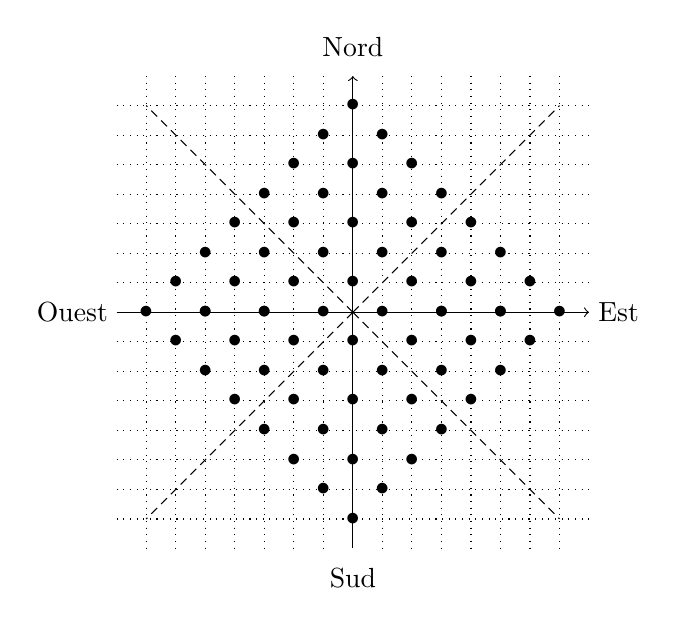
\begin{tikzpicture}[scale=0.375]
\node (n0)    at (-9.5,0)      {Ouest};
\node (n0)    at (9,0)      {Est};
\node (n0)    at (0,-9)      {Sud};
\node (n0)    at (0,9)      {Nord};

\node (n0)    at (0,1)      {$\bullet$};
\node (n0)    at (0,3)      {$\bullet$};
\node (n0)    at (0,5)      {$\bullet$};
\node (n0)    at (0,7)      {$\bullet$};
\node (n0)    at (0,-1)      {$\bullet$};
\node (n0)    at (0,-3)      {$\bullet$};
\node (n0)    at (0,-5)      {$\bullet$};
\node (n0)    at (0,-7)      {$\bullet$};

\node (n0)    at (1,0)      {$\bullet$};
\node (n0)    at (3,0)      {$\bullet$};
\node (n0)    at (5,0)      {$\bullet$};
\node (n0)    at (7,0)      {$\bullet$};
\node (n0)    at (-1,0)      {$\bullet$};
\node (n0)    at (-3,0)      {$\bullet$};
\node (n0)    at (-5,0)      {$\bullet$};
\node (n0)    at (-7,0)      {$\bullet$};

\node (n0)    at (1,2)      {$\bullet$};
\node (n0)    at (1,4)      {$\bullet$};
\node (n0)    at (1,6)      {$\bullet$};
\node (n0)    at (1,-2)      {$\bullet$};
\node (n0)    at (1,-4)      {$\bullet$};
\node (n0)    at (1,-6)      {$\bullet$};
\node (n0)    at (-1,2)      {$\bullet$};
\node (n0)    at (-1,4)      {$\bullet$};
\node (n0)    at (-1,6)      {$\bullet$};
\node (n0)    at (-1,-2)      {$\bullet$};
\node (n0)    at (-1,-4)      {$\bullet$};
\node (n0)    at (-1,-6)      {$\bullet$};

\node (n0)    at (2,1)      {$\bullet$};
\node (n0)    at (2,3)      {$\bullet$};
\node (n0)    at (2,5)      {$\bullet$};
\node (n0)    at (2,-1)      {$\bullet$};
\node (n0)    at (2,-3)      {$\bullet$};
\node (n0)    at (2,-5)      {$\bullet$};
\node (n0)    at (-2,1)      {$\bullet$};
\node (n0)    at (-2,3)      {$\bullet$};
\node (n0)    at (-2,5)      {$\bullet$};
\node (n0)    at (-2,-1)      {$\bullet$};
\node (n0)    at (-2,-3)      {$\bullet$};
\node (n0)    at (-2,-5)      {$\bullet$};

\node (n0)    at (3,0)      {$\bullet$};
\node (n0)    at (3,2)      {$\bullet$};
\node (n0)    at (3,4)      {$\bullet$};
\node (n0)    at (3,-2)      {$\bullet$};
\node (n0)    at (3,-4)      {$\bullet$};
\node (n0)    at (-3,0)      {$\bullet$};
\node (n0)    at (-3,2)      {$\bullet$};
\node (n0)    at (-3,4)      {$\bullet$};
\node (n0)    at (-3,-2)      {$\bullet$};
\node (n0)    at (-3,-4)      {$\bullet$};

\node (n0)    at (4,1)      {$\bullet$};
\node (n0)    at (4,3)      {$\bullet$};
\node (n0)    at (4,-1)      {$\bullet$};
\node (n0)    at (4,-3)      {$\bullet$};
\node (n0)    at (-4,1)      {$\bullet$};
\node (n0)    at (-4,3)      {$\bullet$};
\node (n0)    at (-4,-1)      {$\bullet$};
\node (n0)    at (-4,-3)      {$\bullet$};

\node (n0)    at (5,0)      {$\bullet$};
\node (n0)    at (5,2)      {$\bullet$};
\node (n0)    at (5,-2)      {$\bullet$};
\node (n0)    at (-5,0)      {$\bullet$};
\node (n0)    at (-5,2)      {$\bullet$};
\node (n0)    at (-5,-2)      {$\bullet$};

\node (n0)    at (6,1)      {$\bullet$};
\node (n0)    at (-6,1)      {$\bullet$};
\node (n0)    at (6,-1)      {$\bullet$};
\node (n0)    at (-6,-1)      {$\bullet$};

%\draw[dotted] (-8,8) --  (-8,-8);
\draw[dotted] (-7,8) --  (-7,-8);
\draw[dotted] (-6,8) --  (-6,-8);
\draw[dotted] (-5,8) --  (-5,-8);
\draw[dotted] (-4,8) --  (-4,-8);
\draw[dotted] (-3,8) --  (-3,-8);
\draw[dotted] (-2,8) --  (-2,-8);
\draw[dotted] (-1,8) --  (-1,-8);
\draw[->] (0,-8) --  (0,8);
\draw[dotted] (1,8) --  (1,-8);
\draw[dotted] (2,8) --  (2,-8);
\draw[dotted] (3,8) --  (3,-8);
\draw[dotted] (4,8) --  (4,-8);
\draw[dotted] (5,8) --  (5,-8);
\draw[dotted] (6,8) --  (6,-8);
\draw[dotted] (7,8) --  (7,-8);
%\draw[dotted] (8,8) --  (8,-8);

%\draw[dotted] (-8,8) --  (8,8);
\draw[dotted] (-8,7) --  (8,7);
\draw[dotted] (-8,6) --  (8,6);
\draw[dotted] (-8,5) --  (8,5);
\draw[dotted] (-8,4) --  (8,4);
\draw[dotted] (-8,3) --  (8,3);
\draw[dotted] (-8,2) --  (8,2);
\draw[dotted] (-8,1) --  (8,1);
\draw[->] (-8,0) --  (8,0);
\draw[dotted] (-8,-1) --  (8,-1);
\draw[dotted] (-8,-2) --  (8,-2);
\draw[dotted] (-8,-3) --  (8,-3);
\draw[dotted] (-8,-4) --  (8,-4);
\draw[dotted] (-8,-5) --  (8,-5);
\draw[dotted] (-8,-6) --  (8,-6);
\draw[dotted] (-8,-7) --  (8,-7);
%\draw[dotted] (-8,-8) --  (8,-8);

\draw[densely dashed] (0,0) -- (7,7);
\draw[densely dashed] (0,0) -- (-7,-7);
\draw[densely dashed] (0,0) -- (7,-7);
\draw[densely dashed] (0,0) -- (-7,7);
\end{tikzpicture}
\end{center}
\caption{Places d'un jardin}\label{lagrille}
\end{figure}

Les termes considérés dans le projet désignent des fleurs positionnées
sur une grille. La figure 1 représente la grille : les points noirs
symbolisent les places où peuvent être disposées les fleurs (il y a au
plus une fleur par place). Chaque place est identifiée par ses
coordonnées (le point $(0,0)$ est au centre de la grille). L'ensemble
des places possibles est donc :

\[
\mathrm{Places}  = \left \{
\begin{array}{c}
(0,7) ,
\\
(-1,6), (1,6) ,
\\
(-2,5) , (0,5) , (2,5),
\\
(-3,4) , (-1,4) , (1,4) , (3,4),
\\
(-4,3), (-2,3), (0,3) , (2,3), (4,3),
\\
(-5,2),(-3,2) , (-1,2) , (1,2) , (3,2), (5,2),
\\
(-6,1),(-4,1), (-2,1), (0,1) , (2,1) , (4,1),(6,1),
\\
(-7,0) , (-5,0) , (-3,0) , (-1,0) , (1,0) , (3,0) , (5,0) , (7,0) ,
\\
(-6,-1),(-4,-1), (-2,-1), (0,-1) , (2,-1), (4,-1),(6,-1),
\\
(-5,-2),(-3,-2), (-1,-2), (1,-2) , (3,-2),(5,-2),
\\
(-4,-3), (-2,-3) , (0,-3) , (2,-3), (4,-3),
\\
(-3,-4), (-1,-4), (1,-4) , (3,-4) ,
\\
(-2,-5) , (0,-5) , (2,-5),
\\
(-1,-6),  (1,-6),
\\
(0,-7)
\\
\end{array}
\right \}
\]

Chaque fleur appartient à une espèce (les roses, les pâquerettes et
les tulipes), est d'une certaine taille (grande, moyenne ou petite) et
d'une certaine couleur (rouge, rose, blanche).

 \[ \begin{array}{l}
   Especes =  \{rose, paquerette,tulipe \}, \\
   Tailles =  \{grand, moyen, petit \},\\
   Couleurs = \{rouge,rose, blanc \}.
\end{array}
\]

Certaines fleurs ont un nom : il s'agit d'une constante de $F_0$ (deux
fleurs différentes ne peuvent pas avoir le même nom). Un jardin $j$
est la donnée d'une grille sur laquelle sont disposées des fleurs
(chaque jardin contient au moins une fleur) et est représentée par une
liste de quintuplets. Chaque quintuplet $((x, y), e, t, c, n) \in j$
est un élément du produit cartésien :

 \begin{center}
 $Places \times Especes \times Tailles \times Couleurs \times(F_0 \cup \left \{None\right \})$ 
 \end{center}
 
\noindent
et exprime qu'une fleur de nom $n$ ($n$ = None si la fleur n'a pas de
nom), d'espèce $e$, de taille $t$ et de couleur $c$ se trouve à la
place $(x, y)$ dans le jardin j. L'ensemble des jardins possibles est
donc :
 
  \begin{center}
  $J = \wp(Places \times Especes \times Tailles \times Couleurs \times(F_0 \cup \left \{None\right \})\setminus\left \{\emptyset\right \}$ 
 \end{center}

%Contenu de la note précédemment marquée avec \footnotemark
%\footnotetext{Note bas de page "intro"}



\newpage

\section{Existant : évaluation des formules}

Le projet tourne autour d'un script préalablement fourni en python.

\subsection{Script python}

Le script permet de créer un jardin en disposant les différents éléments avec leurs attributs sur diverses coordonnées.
En premier lieu il est nécessaire de bien créer un jardin, il serait inutile de tester une formule sans contexte autour.
Le script permet ensuite de créer une formule, celle-ci doit être préalablement vérifiée pour que sa syntaxe ne contienne aucune erreur.
Dans un dernier temps le script analyse la formule dans le contexte du jardin donné et retourne un booléen en résultat.


\subsection{Bilan récapitulatif}

En résumé ce script python permet de :
\begin{itemize}
\item Construire un jardin en ligne de code
\item Construire une formule en ligne de code
\item Analyser si une formule est cohérente pour un jardin donnée et inversement.
\end{itemize}

Les enjeux majeurs de ce projet sont alors de pouvoir :
\begin{itemize}
\item Construire un jardin graphiquement
\item Construire une formule graphiquement (avec un clavier virtuel)
\item Vérifier qu'une formule est syntaxiquement correcte
\item Faire communiquer les points ci-dessus avec le script python
\end{itemize}

%Voici le tableau (cf. fig. 2.1) récapitulatif de l'analyse de l'existant:\\

%tableau centré à taille variable qui s'ajuste automatiquement suivant la longueur du contenu
%\begin{figure}[!h]
%\begin{center}
%\begin{tabular}{|l|l|l|l|}
%  \hline
%  Solution & Création & Vérification & Analyse\\
%  \hline
%  Jardin & Oui & Non & Non \\
%  Formule & Oui & Non & Oui \\
%  \hline
%\end{tabular}
%\end{center}
%\caption{Tableau récapitulatif des solutions}
%\end{figure}

\section{Problématiques soulevées}

Deux problématiques importantes sont alors soulevées pour la réalisation de ce projet.
\begin{itemize}
\item La récupération et vérification de l'intégrité syntaxique des formules entrées dans le programme avant de les envoyer au script de vérification de leur véracité dans un jardin donné;
\item La communication entre deux langages différents et une interface graphique.
\end{itemize}

\section{Hypothèse de solution}

%Quoi :
\subsection{Problématique de l'intégrité syntaxique}

%Comment :
La solution envisagée est l'utilisation d'un générateur d'analyseur syntaxique, idéalement via l'outil Grammatica version 1.6 (libre de droit sous licence BSD). Après que l'outil ait reçu une grammaire spécifique
en entrée, il produit un parseur pour cette grammaire en C\#. Ce code
n'est généré qu'une seule fois et est capable d'analyser des formules
données sous forme de chaînes de caractères. Le résultat final obtenu
est soit un message d'erreur détaillé si la formule est incorrecte
soit un arbre syntaxique représenté en C\# comme l'illustre la figure 1.2.


\begin{figure}[!ht]
\begin{center}
\includegraphics[height=7cm]{presentation/syntaxtree}
\end{center}
\caption[schema]{Analyse syntaxique}
\end{figure}

%Detail :
%citation référencé dans le document "bibliographie.bib" inclus à la fin du document

%Quoi :
\subsection{Problématique de la communication}

%Comment :
Le sujet du projet est fourni avec un script de vérification des formules. Il est donc important de pouvoir faire communiquer ce script avec le langage de développement choisi: C\#, ainsi qu'avec les briques fournies par l'API de Unity.
Ainsi la communication symbolise la brique liante entre la partie syntaxique, le script de vérification, et les entrées utilisateur via l'interface graphique.

%Detail :
%citation référencé dans le document "bibliographie.bib" inclus à la fin du document